\documentclass{BHCexam}
\begin{document}
%	\begin{minipage}[b]{0.7\textwidth}
%		\flushright
%		dfssgag测试问题地方得分都是收费的沙发上飞洒发上市公司感受过是多个点供电公司发生过个
%		是的归属感是个十个`$12 $`感受过是个十个闪电告诉
%	\end{minipage}\hspace{2em}
%	\begin{minipage}[b]{0.28\textwidth}
%		dfssgag测试问题地方得分都是收费的沙发上飞洒发上市公司感受过是多个点供电公司发生过个
%	是的归属感是个十个`$12 $`感受过是个十个闪电告诉
%\end{minipage}
\begin{questions}
	\begin{minipage}[b]{0.7\textwidth}
		\qs 若$ 0<x_1<x_2<1 $,则\xx
	\twoch{$ \mathrm{e}^{x_2}-\mathrm{e}^{x_1}>\ln{x_2}-\ln{x_1}$}{$\mathrm{e}^{x_2}-\mathrm{e}^{x_1}<\ln{x_2}-\ln{x_1} $}{$ x_2\mathrm{e}^{x_1}>x_1\mathrm{e}^{x_2}$}{$x_2\mathrm{e}^{x_1}<x_1\mathrm{e}^{x_2} $}
	\end{minipage}
\begin{minipage}[h]{0.25\textwidth}
	
	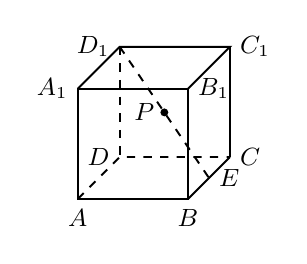
\begin{tikzpicture}[line width=0.7 pt,scale=0.7]
	%\draw[help lines] (0,0) grid (3,3);
	\draw (0,0) node[below](A) {\small$A$}--(2,0) node[below](B){\small$B$}--(2,2) node[right](B1){\small$B_1$}--(0,2) node[left](A1) {\small$A_1$}--(0,0)--cycle;
	\draw[dashed] (0,0)--(0.76,0.76) node[left](D){\small$D$}--(2.76,0.76) node[right](C){\small$C$};
	\draw (2.76,0.76)--(2,0);
	\draw (0,2) --(0.76,2.76)node[left](D1){\small$D_1$}--(2.76,2.76)node[right](C1){\small$C_1$}--(2,2);
	\draw [dashed](0.76,2.76)--(0.76,0.76) ;
	\draw (2.76,2.76)--(2.76,0.76);
	\draw [dashed](0.76,2.76)--(2.38,0.38) node[right](E) {\small$E$};
	\coordinate[label=left:\small$P$] (P) at (1.57,1.57);
	\draw[fill] (P) circle (1.5pt) ;
	\end{tikzpicture}
\end{minipage}
\begin{tikzpicture}[x={(-0.1cm,-0.15cm)},y={(1cm,0cm)},z={(0cm,1cm)}]
\draw(0,0)--(3,0,0) node(x) {$x$};
	\draw(0,0)--(0,1,0) node(y) {$y$};
	\draw(0,0)--(0,0,1) node(z) {$z$};

\end{tikzpicture}
\end{questions}
\end{document}